\documentclass[1p]{elsarticle_modified}
%\bibliographystyle{elsarticle-num}

%\usepackage[colorlinks]{hyperref}
%\usepackage{abbrmath_seonhwa} %\Abb, \Ascr, \Acal ,\Abf, \Afrak
\usepackage{amsfonts}
\usepackage{amssymb}
\usepackage{amsmath}
\usepackage{amsthm}
\usepackage{scalefnt}
\usepackage{amsbsy}
\usepackage{kotex}
\usepackage{caption}
\usepackage{subfig}
\usepackage{color}
\usepackage{graphicx}
\usepackage{xcolor} %% white, black, red, green, blue, cyan, magenta, yellow
\usepackage{float}
\usepackage{setspace}
\usepackage{hyperref}

\usepackage{tikz}
\usetikzlibrary{arrows}

\usepackage{multirow}
\usepackage{array} % fixed length table
\usepackage{hhline}

%%%%%%%%%%%%%%%%%%%%%
\makeatletter
\renewcommand*\env@matrix[1][\arraystretch]{%
	\edef\arraystretch{#1}%
	\hskip -\arraycolsep
	\let\@ifnextchar\new@ifnextchar
	\array{*\c@MaxMatrixCols c}}
\makeatother %https://tex.stackexchange.com/questions/14071/how-can-i-increase-the-line-spacing-in-a-matrix
%%%%%%%%%%%%%%%

\usepackage[normalem]{ulem}

\newcommand{\msout}[1]{\ifmmode\text{\sout{\ensuremath{#1}}}\else\sout{#1}\fi}
%SOURCE: \msout is \stkout macro in https://tex.stackexchange.com/questions/20609/strikeout-in-math-mode

\newcommand{\cancel}[1]{
	\ifmmode
	{\color{red}\msout{#1}}
	\else
	{\color{red}\sout{#1}}
	\fi
}

\newcommand{\add}[1]{
	{\color{blue}\uwave{#1}}
}

\newcommand{\replace}[2]{
	\ifmmode
	{\color{red}\msout{#1}}{\color{blue}\uwave{#2}}
	\else
	{\color{red}\sout{#1}}{\color{blue}\uwave{#2}}
	\fi
}

\newcommand{\Sol}{\mathcal{S}} %segment
\newcommand{\D}{D} %diagram
\newcommand{\A}{\mathcal{A}} %arc


%%%%%%%%%%%%%%%%%%%%%%%%%%%%%5 test

\def\sl{\operatorname{\textup{SL}}(2,\Cbb)}
\def\psl{\operatorname{\textup{PSL}}(2,\Cbb)}
\def\quan{\mkern 1mu \triangleright \mkern 1mu}

\theoremstyle{definition}
\newtheorem{thm}{Theorem}[section]
\newtheorem{prop}[thm]{Proposition}
\newtheorem{lem}[thm]{Lemma}
\newtheorem{ques}[thm]{Question}
\newtheorem{cor}[thm]{Corollary}
\newtheorem{defn}[thm]{Definition}
\newtheorem{exam}[thm]{Example}
\newtheorem{rmk}[thm]{Remark}
\newtheorem{alg}[thm]{Algorithm}

\newcommand{\I}{\sqrt{-1}}
\begin{document}

%\begin{frontmatter}
%
%\title{Boundary parabolic representations of knots up to 8 crossings}
%
%%% Group authors per affiliation:
%\author{Yunhi Cho} 
%\address{Department of Mathematics, University of Seoul, Seoul, Korea}
%\ead{yhcho@uos.ac.kr}
%
%
%\author{Seonhwa Kim} %\fnref{s_kim}}
%\address{Center for Geometry and Physics, Institute for Basic Science, Pohang, 37673, Korea}
%\ead{ryeona17@ibs.re.kr}
%
%\author{Hyuk Kim}
%\address{Department of Mathematical Sciences, Seoul National University, Seoul 08826, Korea}
%\ead{hyukkim@snu.ac.kr}
%
%\author{Seokbeom Yoon}
%\address{Department of Mathematical Sciences, Seoul National University, Seoul, 08826,  Korea}
%\ead{sbyoon15@snu.ac.kr}
%
%\begin{abstract}
%We find all boundary parabolic representation of knots up to 8 crossings.
%
%\end{abstract}
%\begin{keyword}
%    \MSC[2010] 57M25 
%\end{keyword}
%
%\end{frontmatter}

%\linenumbers
%\tableofcontents
%
\newcommand\colored[1]{\textcolor{white}{\rule[-0.35ex]{0.8em}{1.4ex}}\kern-0.8em\color{red} #1}%
%\newcommand\colored[1]{\textcolor{white}{ #1}\kern-2.17ex	\textcolor{white}{ #1}\kern-1.81ex	\textcolor{white}{ #1}\kern-2.15ex\color{red}#1	}

{\Large $\underline{12n_{0415}~(K12n_{0415})}$}

\setlength{\tabcolsep}{10pt}
\renewcommand{\arraystretch}{1.6}
\vspace{1cm}\begin{tabular}{m{100pt}>{\centering\arraybackslash}m{274pt}}
\multirow{5}{120pt}{
	\centering
	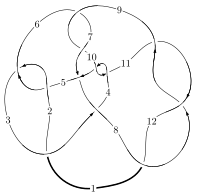
\includegraphics[width=112pt]{../../../GIT/diagram.site/Diagrams/png/2504_12n_0415.png}\\
\ \ \ A knot diagram\footnotemark}&
\allowdisplaybreaks
\textbf{Linearized knot diagam} \\
\cline{2-2}
 &
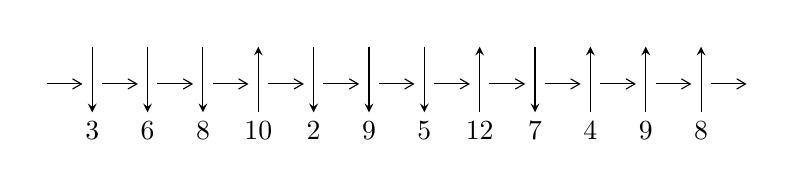
\begin{tikzpicture}[x=20pt, y=17pt]
	% nodes
	\node (C0) at (0, 0) {};
	\node (C1) at (1, 0) {};
	\node (C1U) at (1, +1) {};
	\node (C1D) at (1, -1) {3};

	\node (C2) at (2, 0) {};
	\node (C2U) at (2, +1) {};
	\node (C2D) at (2, -1) {6};

	\node (C3) at (3, 0) {};
	\node (C3U) at (3, +1) {};
	\node (C3D) at (3, -1) {8};

	\node (C4) at (4, 0) {};
	\node (C4U) at (4, +1) {};
	\node (C4D) at (4, -1) {10};

	\node (C5) at (5, 0) {};
	\node (C5U) at (5, +1) {};
	\node (C5D) at (5, -1) {2};

	\node (C6) at (6, 0) {};
	\node (C6U) at (6, +1) {};
	\node (C6D) at (6, -1) {9};

	\node (C7) at (7, 0) {};
	\node (C7U) at (7, +1) {};
	\node (C7D) at (7, -1) {5};

	\node (C8) at (8, 0) {};
	\node (C8U) at (8, +1) {};
	\node (C8D) at (8, -1) {12};

	\node (C9) at (9, 0) {};
	\node (C9U) at (9, +1) {};
	\node (C9D) at (9, -1) {7};

	\node (C10) at (10, 0) {};
	\node (C10U) at (10, +1) {};
	\node (C10D) at (10, -1) {4};

	\node (C11) at (11, 0) {};
	\node (C11U) at (11, +1) {};
	\node (C11D) at (11, -1) {9};

	\node (C12) at (12, 0) {};
	\node (C12U) at (12, +1) {};
	\node (C12D) at (12, -1) {8};
	\node (C13) at (13, 0) {};

	% arrows
	\draw[->,>={angle 60}]
	(C0) edge (C1) (C1) edge (C2) (C2) edge (C3) (C3) edge (C4) (C4) edge (C5) (C5) edge (C6) (C6) edge (C7) (C7) edge (C8) (C8) edge (C9) (C9) edge (C10) (C10) edge (C11) (C11) edge (C12) (C12) edge (C13) ;	\draw[->,>=stealth]
	(C1U) edge (C1D) (C2U) edge (C2D) (C3U) edge (C3D) (C4D) edge (C4U) (C5U) edge (C5D) (C6U) edge (C6D) (C7U) edge (C7D) (C8D) edge (C8U) (C9U) edge (C9D) (C10D) edge (C10U) (C11D) edge (C11U) (C12D) edge (C12U) ;
	\end{tikzpicture} \\
\hhline{~~} \\& 
\textbf{Solving Sequence} \\ \cline{2-2} 
 &
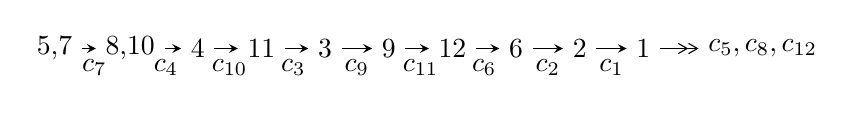
\begin{tikzpicture}[x=23pt, y=7pt]
	% node
	\node (A0) at (-1/8, 0) {5,7};
	\node (A1) at (17/16, 0) {8,10};
	\node (A2) at (17/8, 0) {4};
	\node (A3) at (25/8, 0) {11};
	\node (A4) at (33/8, 0) {3};
	\node (A5) at (41/8, 0) {9};
	\node (A6) at (49/8, 0) {12};
	\node (A7) at (57/8, 0) {6};
	\node (A8) at (65/8, 0) {2};
	\node (A9) at (73/8, 0) {1};
	\node (C1) at (1/2, -1) {$c_{7}$};
	\node (C2) at (13/8, -1) {$c_{4}$};
	\node (C3) at (21/8, -1) {$c_{10}$};
	\node (C4) at (29/8, -1) {$c_{3}$};
	\node (C5) at (37/8, -1) {$c_{9}$};
	\node (C6) at (45/8, -1) {$c_{11}$};
	\node (C7) at (53/8, -1) {$c_{6}$};
	\node (C8) at (61/8, -1) {$c_{2}$};
	\node (C9) at (69/8, -1) {$c_{1}$};
	\node (A10) at (11, 0) {$c_{5},c_{8},c_{12}$};

	% edge
	\draw[->,>=stealth]	
	(A0) edge (A1) (A1) edge (A2) (A2) edge (A3) (A3) edge (A4) (A4) edge (A5) (A5) edge (A6) (A6) edge (A7) (A7) edge (A8) (A8) edge (A9) ;
	\draw[->>,>={angle 60}]	
	(A9) edge (A10);
\end{tikzpicture} \\ 

\end{tabular} \\

\footnotetext{
The image of knot diagram is generated by the software ``\textbf{Draw programme}" developed by Andrew Bartholomew(\url{http://www.layer8.co.uk/maths/draw/index.htm\#Running-draw}), where we modified some parts for our purpose(\url{https://github.com/CATsTAILs/LinksPainter}).
}\phantom \\ \newline 
\centering \textbf{Ideals for irreducible components\footnotemark of $X_{\text{par}}$} 
 
\begin{align*}
I^u_{1}&=\langle 
2.62328\times10^{249} u^{73}-7.69335\times10^{248} u^{72}+\cdots+6.16724\times10^{251} b+2.89562\times10^{253},\\
\phantom{I^u_{1}}&\phantom{= \langle  }3.89167\times10^{253} u^{73}+3.50798\times10^{253} u^{72}+\cdots+1.76568\times10^{255} a+6.42586\times10^{256},\\
\phantom{I^u_{1}}&\phantom{= \langle  }u^{74}-18 u^{72}+\cdots+13014 u-2863\rangle \\
I^u_{2}&=\langle 
1461328095574788 u^{22}+4128500756671431 u^{21}+\cdots+2694132033228847 b+3183360713386177,\\
\phantom{I^u_{2}}&\phantom{= \langle  }1596568487678737 u^{22}+4700269669705836 u^{21}+\cdots+2694132033228847 a+3243990326400528,\\
\phantom{I^u_{2}}&\phantom{= \langle  }u^{23}+3 u^{22}+\cdots+6 u+1\rangle \\
\\
\end{align*}
\raggedright * 2 irreducible components of $\dim_{\mathbb{C}}=0$, with total 97 representations.\\
\footnotetext{All coefficients of polynomials are rational numbers. But the coefficients are sometimes approximated in decimal forms when there is not enough margin.}
\newpage
\renewcommand{\arraystretch}{1}
\centering \section*{I. $I^u_{1}= \langle 2.62\times10^{249} u^{73}-7.69\times10^{248} u^{72}+\cdots+6.17\times10^{251} b+2.90\times10^{253},\;3.89\times10^{253} u^{73}+3.51\times10^{253} u^{72}+\cdots+1.77\times10^{255} a+6.43\times10^{256},\;u^{74}-18 u^{72}+\cdots+13014 u-2863 \rangle$}
\flushleft \textbf{(i) Arc colorings}\\
\begin{tabular}{m{7pt} m{180pt} m{7pt} m{180pt} }
\flushright $a_{5}=$&$\begin{pmatrix}0\\u\end{pmatrix}$ \\
\flushright $a_{7}=$&$\begin{pmatrix}1\\0\end{pmatrix}$ \\
\flushright $a_{8}=$&$\begin{pmatrix}1\\u^2\end{pmatrix}$ \\
\flushright $a_{10}=$&$\begin{pmatrix}-0.0220406 u^{73}-0.0198675 u^{72}+\cdots+220.643 u-36.3930\\-0.00425356 u^{73}+0.00124745 u^{72}+\cdots+110.198 u-46.9517\end{pmatrix}$ \\
\flushright $a_{4}=$&$\begin{pmatrix}-0.0000705915 u^{73}-0.00699554 u^{72}+\cdots-79.9649 u+50.6943\\-0.00337096 u^{73}-0.00295357 u^{72}+\cdots+37.0277 u-13.3009\end{pmatrix}$ \\
\flushright $a_{11}=$&$\begin{pmatrix}0.0523964 u^{73}+0.0340422 u^{72}+\cdots-668.716 u+180.347\\0.00944346 u^{73}-0.00258887 u^{72}+\cdots-230.912 u+91.9988\end{pmatrix}$ \\
\flushright $a_{3}=$&$\begin{pmatrix}0.00494268 u^{73}-0.00257029 u^{72}+\cdots-133.775 u+57.4216\\-0.000435248 u^{73}-0.00119965 u^{72}+\cdots-6.20955 u-0.631443\end{pmatrix}$ \\
\flushright $a_{9}=$&$\begin{pmatrix}-0.0262941 u^{73}-0.0186201 u^{72}+\cdots+330.841 u-83.3447\\-0.00425356 u^{73}+0.00124745 u^{72}+\cdots+110.198 u-46.9517\end{pmatrix}$ \\
\flushright $a_{12}=$&$\begin{pmatrix}0.0478425 u^{73}+0.0317582 u^{72}+\cdots-609.789 u+166.141\\0.00647358 u^{73}-0.00178615 u^{72}+\cdots-156.506 u+66.0267\end{pmatrix}$ \\
\flushright $a_{6}=$&$\begin{pmatrix}-0.0105705 u^{73}-0.00873866 u^{72}+\cdots+119.067 u-31.9627\\-0.00592470 u^{73}-0.00536770 u^{72}+\cdots+55.6302 u-8.52990\end{pmatrix}$ \\
\flushright $a_{2}=$&$\begin{pmatrix}0.00824933 u^{73}+0.00495099 u^{72}+\cdots-115.733 u+38.0504\\0.00567037 u^{73}+0.00516383 u^{72}+\cdots-56.2245 u+5.68267\end{pmatrix}$ \\
\flushright $a_{1}=$&$\begin{pmatrix}-0.0375306 u^{73}-0.0237185 u^{72}+\cdots+489.967 u-141.244\\-0.00173001 u^{73}+0.00381214 u^{72}+\cdots+81.4010 u-43.0091\end{pmatrix}$\\&\end{tabular}
\flushleft \textbf{(ii) Obstruction class $= -1$}\\~\\
\flushleft \textbf{(iii) Cusp Shapes $= 0.0209656 u^{73}+0.000371330 u^{72}+\cdots-411.018 u+116.524$}\\~\\
\newpage\renewcommand{\arraystretch}{1}
\flushleft \textbf{(iv) u-Polynomials at the component}\newline \\
\begin{tabular}{m{50pt}|m{274pt}}
Crossings & \hspace{64pt}u-Polynomials at each crossing \\
\hline $$\begin{aligned}c_{1}\end{aligned}$$&$\begin{aligned}
&u^{74}+24 u^{73}+\cdots+43970 u+2209
\end{aligned}$\\
\hline $$\begin{aligned}c_{2},c_{5}\end{aligned}$$&$\begin{aligned}
&u^{74}+4 u^{73}+\cdots+52 u+47
\end{aligned}$\\
\hline $$\begin{aligned}c_{3}\end{aligned}$$&$\begin{aligned}
&u^{74}+29 u^{72}+\cdots-70400 u-24287
\end{aligned}$\\
\hline $$\begin{aligned}c_{4},c_{10}\end{aligned}$$&$\begin{aligned}
&u^{74}+3 u^{73}+\cdots-43360 u-4517
\end{aligned}$\\
\hline $$\begin{aligned}c_{6},c_{9}\end{aligned}$$&$\begin{aligned}
&u^{74}+3 u^{73}+\cdots-132 u+2447
\end{aligned}$\\
\hline $$\begin{aligned}c_{7}\end{aligned}$$&$\begin{aligned}
&u^{74}-18 u^{72}+\cdots+13014 u-2863
\end{aligned}$\\
\hline $$\begin{aligned}c_{8},c_{11},c_{12}\end{aligned}$$&$\begin{aligned}
&u^{74}+4 u^{73}+\cdots-148 u-7
\end{aligned}$\\
\hline
\end{tabular}\\~\\
\newpage\renewcommand{\arraystretch}{1}
\flushleft \textbf{(v) Riley Polynomials at the component}\newline \\
\begin{tabular}{m{50pt}|m{274pt}}
Crossings & \hspace{64pt}Riley Polynomials at each crossing \\
\hline $$\begin{aligned}c_{1}\end{aligned}$$&$\begin{aligned}
&y^{74}+64 y^{73}+\cdots-202684506 y+4879681
\end{aligned}$\\
\hline $$\begin{aligned}c_{2},c_{5}\end{aligned}$$&$\begin{aligned}
&y^{74}-24 y^{73}+\cdots-43970 y+2209
\end{aligned}$\\
\hline $$\begin{aligned}c_{3}\end{aligned}$$&$\begin{aligned}
&y^{74}+58 y^{73}+\cdots-49646717274 y+589858369
\end{aligned}$\\
\hline $$\begin{aligned}c_{4},c_{10}\end{aligned}$$&$\begin{aligned}
&y^{74}+43 y^{73}+\cdots+78391260 y+20403289
\end{aligned}$\\
\hline $$\begin{aligned}c_{6},c_{9}\end{aligned}$$&$\begin{aligned}
&y^{74}-39 y^{73}+\cdots-103437432 y+5987809
\end{aligned}$\\
\hline $$\begin{aligned}c_{7}\end{aligned}$$&$\begin{aligned}
&y^{74}-36 y^{73}+\cdots-172879960 y+8196769
\end{aligned}$\\
\hline $$\begin{aligned}c_{8},c_{11},c_{12}\end{aligned}$$&$\begin{aligned}
&y^{74}+26 y^{73}+\cdots-6546 y+49
\end{aligned}$\\
\hline
\end{tabular}\\~\\
\newpage\flushleft \textbf{(vi) Complex Volumes and Cusp Shapes}
$$\begin{array}{c|c|c}  
\text{Solutions to }I^u_{1}& \I (\text{vol} + \sqrt{-1}CS) & \text{Cusp shape}\\
 \hline 
\begin{aligned}
u &= -0.716939 + 0.702052 I \\
a &= \phantom{-}0.30263 - 1.41247 I \\
b &= -1.177540 + 0.285975 I\end{aligned}
 & -1.91366 + 4.24234 I & \phantom{-0.000000 } 0 \\ \hline\begin{aligned}
u &= -0.716939 - 0.702052 I \\
a &= \phantom{-}0.30263 + 1.41247 I \\
b &= -1.177540 - 0.285975 I\end{aligned}
 & -1.91366 - 4.24234 I & \phantom{-0.000000 } 0 \\ \hline\begin{aligned}
u &= \phantom{-}0.816631 + 0.612281 I \\
a &= -0.145660 - 1.130310 I \\
b &= -0.396070 + 1.216810 I\end{aligned}
 & \phantom{-}4.09032 - 3.11910 I & \phantom{-0.000000 } 0 \\ \hline\begin{aligned}
u &= \phantom{-}0.816631 - 0.612281 I \\
a &= -0.145660 + 1.130310 I \\
b &= -0.396070 - 1.216810 I\end{aligned}
 & \phantom{-}4.09032 + 3.11910 I & \phantom{-0.000000 } 0 \\ \hline\begin{aligned}
u &= -0.725639 + 0.606653 I \\
a &= -1.35528 - 0.64131 I \\
b &= -0.947841 + 0.475507 I\end{aligned}
 & \phantom{-}4.37251 + 2.51666 I & \phantom{-0.000000 } 0. - 3.92703 I \\ \hline\begin{aligned}
u &= -0.725639 - 0.606653 I \\
a &= -1.35528 + 0.64131 I \\
b &= -0.947841 - 0.475507 I\end{aligned}
 & \phantom{-}4.37251 - 2.51666 I & \phantom{-0.000000 -}0. + 3.92703 I \\ \hline\begin{aligned}
u &= -0.852419 + 0.625156 I \\
a &= \phantom{-}1.304660 - 0.001023 I \\
b &= \phantom{-}0.820732 - 0.436023 I\end{aligned}
 & \phantom{-}3.15839 - 4.36525 I & \phantom{-0.000000 } 0 \\ \hline\begin{aligned}
u &= -0.852419 - 0.625156 I \\
a &= \phantom{-}1.304660 + 0.001023 I \\
b &= \phantom{-}0.820732 + 0.436023 I\end{aligned}
 & \phantom{-}3.15839 + 4.36525 I & \phantom{-0.000000 } 0 \\ \hline\begin{aligned}
u &= -0.673467 + 0.818072 I \\
a &= \phantom{-}1.06661 - 1.08020 I \\
b &= -0.880323 + 0.113571 I\end{aligned}
 & -3.27559 + 3.44834 I & \phantom{-0.000000 } 0 \\ \hline\begin{aligned}
u &= -0.673467 - 0.818072 I \\
a &= \phantom{-}1.06661 + 1.08020 I \\
b &= -0.880323 - 0.113571 I\end{aligned}
 & -3.27559 - 3.44834 I & \phantom{-0.000000 } 0\\
 \hline 
 \end{array}$$\newpage$$\begin{array}{c|c|c}  
\text{Solutions to }I^u_{1}& \I (\text{vol} + \sqrt{-1}CS) & \text{Cusp shape}\\
 \hline 
\begin{aligned}
u &= \phantom{-}1.06373\phantom{ +0.000000I} \\
a &= \phantom{-}1.17437\phantom{ +0.000000I} \\
b &= \phantom{-}0.718671\phantom{ +0.000000I}\end{aligned}
 & -0.362734\phantom{ +0.000000I} & -17.0640\phantom{ +0.000000I} \\ \hline\begin{aligned}
u &= -0.903098 + 0.592548 I \\
a &= -0.266612 + 0.712330 I \\
b &= \phantom{-}1.281040 - 0.243461 I\end{aligned}
 & -2.73174 + 0.73218 I & \phantom{-0.000000 } 0 \\ \hline\begin{aligned}
u &= -0.903098 - 0.592548 I \\
a &= -0.266612 - 0.712330 I \\
b &= \phantom{-}1.281040 + 0.243461 I\end{aligned}
 & -2.73174 - 0.73218 I & \phantom{-0.000000 } 0 \\ \hline\begin{aligned}
u &= \phantom{-}0.985502 + 0.449873 I \\
a &= -0.196631 - 0.931982 I \\
b &= \phantom{-}1.55766 + 0.61167 I\end{aligned}
 & -6.28650 - 4.67409 I & \phantom{-0.000000 } 0 \\ \hline\begin{aligned}
u &= \phantom{-}0.985502 - 0.449873 I \\
a &= -0.196631 + 0.931982 I \\
b &= \phantom{-}1.55766 - 0.61167 I\end{aligned}
 & -6.28650 + 4.67409 I & \phantom{-0.000000 } 0 \\ \hline\begin{aligned}
u &= -0.640773 + 0.884634 I \\
a &= -0.861652 + 0.852553 I \\
b &= \phantom{-}1.057100 - 0.700305 I\end{aligned}
 & -5.13856 + 5.00397 I & \phantom{-0.000000 } 0 \\ \hline\begin{aligned}
u &= -0.640773 - 0.884634 I \\
a &= -0.861652 - 0.852553 I \\
b &= \phantom{-}1.057100 + 0.700305 I\end{aligned}
 & -5.13856 - 5.00397 I & \phantom{-0.000000 } 0 \\ \hline\begin{aligned}
u &= -0.948790 + 0.566130 I \\
a &= -0.138082 + 1.073610 I \\
b &= -0.42227 - 1.37744 I\end{aligned}
 & \phantom{-}2.82069 + 9.00069 I & \phantom{-0.000000 } 0 \\ \hline\begin{aligned}
u &= -0.948790 - 0.566130 I \\
a &= -0.138082 - 1.073610 I \\
b &= -0.42227 + 1.37744 I\end{aligned}
 & \phantom{-}2.82069 - 9.00069 I & \phantom{-0.000000 } 0 \\ \hline\begin{aligned}
u &= \phantom{-}0.707873 + 0.524027 I \\
a &= -0.579354 - 0.901201 I \\
b &= \phantom{-}1.55178 - 0.11686 I\end{aligned}
 & -6.09027 + 3.52399 I & -9.61885 - 4.91747 I\\
 \hline 
 \end{array}$$\newpage$$\begin{array}{c|c|c}  
\text{Solutions to }I^u_{1}& \I (\text{vol} + \sqrt{-1}CS) & \text{Cusp shape}\\
 \hline 
\begin{aligned}
u &= \phantom{-}0.707873 - 0.524027 I \\
a &= -0.579354 + 0.901201 I \\
b &= \phantom{-}1.55178 + 0.11686 I\end{aligned}
 & -6.09027 - 3.52399 I & -9.61885 + 4.91747 I \\ \hline\begin{aligned}
u &= \phantom{-}0.923459 + 0.638543 I \\
a &= -1.161220 + 0.518619 I \\
b &= -1.000280 - 0.498046 I\end{aligned}
 & \phantom{-}3.46828 - 9.04581 I & \phantom{-0.000000 } 0 \\ \hline\begin{aligned}
u &= \phantom{-}0.923459 - 0.638543 I \\
a &= -1.161220 - 0.518619 I \\
b &= -1.000280 + 0.498046 I\end{aligned}
 & \phantom{-}3.46828 + 9.04581 I & \phantom{-0.000000 } 0 \\ \hline\begin{aligned}
u &= \phantom{-}0.987910 + 0.559553 I \\
a &= \phantom{-}1.248430 - 0.014833 I \\
b &= \phantom{-}0.823741 + 0.340152 I\end{aligned}
 & \phantom{-}3.57201 - 1.47959 I & \phantom{-0.000000 } 0 \\ \hline\begin{aligned}
u &= \phantom{-}0.987910 - 0.559553 I \\
a &= \phantom{-}1.248430 + 0.014833 I \\
b &= \phantom{-}0.823741 - 0.340152 I\end{aligned}
 & \phantom{-}3.57201 + 1.47959 I & \phantom{-0.000000 } 0 \\ \hline\begin{aligned}
u &= \phantom{-}0.877611 + 0.726426 I \\
a &= \phantom{-}0.042974 + 0.803893 I \\
b &= \phantom{-}0.695871 - 1.040800 I\end{aligned}
 & \phantom{-}3.64324 + 3.84902 I & \phantom{-0.000000 } 0 \\ \hline\begin{aligned}
u &= \phantom{-}0.877611 - 0.726426 I \\
a &= \phantom{-}0.042974 - 0.803893 I \\
b &= \phantom{-}0.695871 + 1.040800 I\end{aligned}
 & \phantom{-}3.64324 - 3.84902 I & \phantom{-0.000000 } 0 \\ \hline\begin{aligned}
u &= \phantom{-}1.103270 + 0.336547 I \\
a &= -0.103428 - 1.230930 I \\
b &= \phantom{-}1.18743 + 0.79431 I\end{aligned}
 & -5.63165 - 5.26461 I & \phantom{-0.000000 } 0 \\ \hline\begin{aligned}
u &= \phantom{-}1.103270 - 0.336547 I \\
a &= -0.103428 + 1.230930 I \\
b &= \phantom{-}1.18743 - 0.79431 I\end{aligned}
 & -5.63165 + 5.26461 I & \phantom{-0.000000 } 0 \\ \hline\begin{aligned}
u &= -0.796570 + 0.190576 I \\
a &= \phantom{-}0.010188 + 1.017090 I \\
b &= \phantom{-}0.211582 - 1.283020 I\end{aligned}
 & -1.99263 + 2.54885 I & -10.22170 - 5.40906 I\\
 \hline 
 \end{array}$$\newpage$$\begin{array}{c|c|c}  
\text{Solutions to }I^u_{1}& \I (\text{vol} + \sqrt{-1}CS) & \text{Cusp shape}\\
 \hline 
\begin{aligned}
u &= -0.796570 - 0.190576 I \\
a &= \phantom{-}0.010188 - 1.017090 I \\
b &= \phantom{-}0.211582 + 1.283020 I\end{aligned}
 & -1.99263 - 2.54885 I & -10.22170 + 5.40906 I \\ \hline\begin{aligned}
u &= -1.066590 + 0.569316 I \\
a &= \phantom{-}0.012147 - 0.814089 I \\
b &= \phantom{-}0.702734 + 1.086420 I\end{aligned}
 & \phantom{-}3.27734 + 2.13042 I & \phantom{-0.000000 } 0 \\ \hline\begin{aligned}
u &= -1.066590 - 0.569316 I \\
a &= \phantom{-}0.012147 + 0.814089 I \\
b &= \phantom{-}0.702734 - 1.086420 I\end{aligned}
 & \phantom{-}3.27734 - 2.13042 I & \phantom{-0.000000 } 0 \\ \hline\begin{aligned}
u &= \phantom{-}0.727771 + 0.217403 I \\
a &= -0.99187 + 1.55253 I \\
b &= -1.219090 + 0.099908 I\end{aligned}
 & -5.53125 + 1.75381 I & -18.7515 + 4.1564 I \\ \hline\begin{aligned}
u &= \phantom{-}0.727771 - 0.217403 I \\
a &= -0.99187 - 1.55253 I \\
b &= -1.219090 - 0.099908 I\end{aligned}
 & -5.53125 - 1.75381 I & -18.7515 - 4.1564 I \\ \hline\begin{aligned}
u &= -0.745350\phantom{ +0.000000I} \\
a &= \phantom{-}0.431663\phantom{ +0.000000I} \\
b &= \phantom{-}0.526516\phantom{ +0.000000I}\end{aligned}
 & -1.12204\phantom{ +0.000000I} & -10.0080\phantom{ +0.000000I} \\ \hline\begin{aligned}
u &= \phantom{-}1.094760 + 0.647316 I \\
a &= \phantom{-}0.029119 + 1.101910 I \\
b &= -1.44938 - 0.46309 I\end{aligned}
 & -7.43280 - 8.42443 I & \phantom{-0.000000 } 0 \\ \hline\begin{aligned}
u &= \phantom{-}1.094760 - 0.647316 I \\
a &= \phantom{-}0.029119 - 1.101910 I \\
b &= -1.44938 + 0.46309 I\end{aligned}
 & -7.43280 + 8.42443 I & \phantom{-0.000000 } 0 \\ \hline\begin{aligned}
u &= -1.151840 + 0.553031 I \\
a &= -0.327823 + 0.995375 I \\
b &= \phantom{-}1.101040 - 0.883548 I\end{aligned}
 & -5.16306 + 2.04636 I & \phantom{-0.000000 } 0 \\ \hline\begin{aligned}
u &= -1.151840 - 0.553031 I \\
a &= -0.327823 - 0.995375 I \\
b &= \phantom{-}1.101040 + 0.883548 I\end{aligned}
 & -5.16306 - 2.04636 I & \phantom{-0.000000 } 0\\
 \hline 
 \end{array}$$\newpage$$\begin{array}{c|c|c}  
\text{Solutions to }I^u_{1}& \I (\text{vol} + \sqrt{-1}CS) & \text{Cusp shape}\\
 \hline 
\begin{aligned}
u &= -0.548937 + 0.402419 I \\
a &= \phantom{-}1.005520 - 0.125825 I \\
b &= \phantom{-}0.161005 - 0.487205 I\end{aligned}
 & -1.59696 + 0.08613 I & -7.31610 - 0.28304 I \\ \hline\begin{aligned}
u &= -0.548937 - 0.402419 I \\
a &= \phantom{-}1.005520 + 0.125825 I \\
b &= \phantom{-}0.161005 + 0.487205 I\end{aligned}
 & -1.59696 - 0.08613 I & -7.31610 + 0.28304 I \\ \hline\begin{aligned}
u &= \phantom{-}0.587757 + 0.294439 I \\
a &= \phantom{-}0.78373 + 2.38110 I \\
b &= -0.958294 - 0.111877 I\end{aligned}
 & -3.68519 + 2.60434 I & -6.57430 - 4.30794 I \\ \hline\begin{aligned}
u &= \phantom{-}0.587757 - 0.294439 I \\
a &= \phantom{-}0.78373 - 2.38110 I \\
b &= -0.958294 + 0.111877 I\end{aligned}
 & -3.68519 - 2.60434 I & -6.57430 + 4.30794 I \\ \hline\begin{aligned}
u &= \phantom{-}0.349150 + 1.296500 I \\
a &= \phantom{-}0.580015 - 0.365543 I \\
b &= -0.649378 + 0.576102 I\end{aligned}
 & \phantom{-}5.27936 + 1.69380 I & \phantom{-0.000000 } 0 \\ \hline\begin{aligned}
u &= \phantom{-}0.349150 - 1.296500 I \\
a &= \phantom{-}0.580015 + 0.365543 I \\
b &= -0.649378 - 0.576102 I\end{aligned}
 & \phantom{-}5.27936 - 1.69380 I & \phantom{-0.000000 } 0 \\ \hline\begin{aligned}
u &= -0.582914 + 1.254360 I \\
a &= \phantom{-}0.522915 + 0.267349 I \\
b &= -0.611014 - 0.628501 I\end{aligned}
 & \phantom{-}4.67633 + 4.65211 I & \phantom{-0.000000 } 0 \\ \hline\begin{aligned}
u &= -0.582914 - 1.254360 I \\
a &= \phantom{-}0.522915 - 0.267349 I \\
b &= -0.611014 + 0.628501 I\end{aligned}
 & \phantom{-}4.67633 - 4.65211 I & \phantom{-0.000000 } 0 \\ \hline\begin{aligned}
u &= \phantom{-}0.512431 + 0.309854 I \\
a &= -1.07215 - 2.01686 I \\
b &= \phantom{-}1.167200 + 0.731529 I\end{aligned}
 & -5.26261 - 1.53830 I & -8.07293 - 0.86476 I \\ \hline\begin{aligned}
u &= \phantom{-}0.512431 - 0.309854 I \\
a &= -1.07215 + 2.01686 I \\
b &= \phantom{-}1.167200 - 0.731529 I\end{aligned}
 & -5.26261 + 1.53830 I & -8.07293 + 0.86476 I\\
 \hline 
 \end{array}$$\newpage$$\begin{array}{c|c|c}  
\text{Solutions to }I^u_{1}& \I (\text{vol} + \sqrt{-1}CS) & \text{Cusp shape}\\
 \hline 
\begin{aligned}
u &= -0.167408 + 0.549877 I \\
a &= \phantom{-}0.176866 + 0.792527 I \\
b &= \phantom{-}0.612175 - 0.774514 I\end{aligned}
 & -0.94767 + 2.37842 I & \phantom{-}1.45207 - 6.62770 I \\ \hline\begin{aligned}
u &= -0.167408 - 0.549877 I \\
a &= \phantom{-}0.176866 - 0.792527 I \\
b &= \phantom{-}0.612175 + 0.774514 I\end{aligned}
 & -0.94767 - 2.37842 I & \phantom{-}1.45207 + 6.62770 I \\ \hline\begin{aligned}
u &= \phantom{-}1.45999 + 0.14673 I \\
a &= -0.257995 + 0.912915 I \\
b &= -0.978818 - 0.301296 I\end{aligned}
 & -9.34243 - 0.54949 I & \phantom{-0.000000 } 0 \\ \hline\begin{aligned}
u &= \phantom{-}1.45999 - 0.14673 I \\
a &= -0.257995 - 0.912915 I \\
b &= -0.978818 + 0.301296 I\end{aligned}
 & -9.34243 + 0.54949 I & \phantom{-0.000000 } 0 \\ \hline\begin{aligned}
u &= \phantom{-}0.357638 + 0.335061 I \\
a &= \phantom{-}0.47848 - 1.58337 I \\
b &= -0.124566 + 0.560482 I\end{aligned}
 & \phantom{-}1.26391 - 1.01316 I & \phantom{-}4.15434 + 2.93912 I \\ \hline\begin{aligned}
u &= \phantom{-}0.357638 - 0.335061 I \\
a &= \phantom{-}0.47848 + 1.58337 I \\
b &= -0.124566 - 0.560482 I\end{aligned}
 & \phantom{-}1.26391 + 1.01316 I & \phantom{-}4.15434 - 2.93912 I \\ \hline\begin{aligned}
u &= -1.33023 + 0.79257 I \\
a &= \phantom{-}0.103633 + 0.876670 I \\
b &= \phantom{-}1.130880 - 0.742570 I\end{aligned}
 & \phantom{-}2.09763 + 2.66972 I & \phantom{-0.000000 } 0 \\ \hline\begin{aligned}
u &= -1.33023 - 0.79257 I \\
a &= \phantom{-}0.103633 - 0.876670 I \\
b &= \phantom{-}1.130880 + 0.742570 I\end{aligned}
 & \phantom{-}2.09763 - 2.66972 I & \phantom{-0.000000 } 0 \\ \hline\begin{aligned}
u &= \phantom{-}1.43130 + 0.70692 I \\
a &= \phantom{-}0.126806 - 0.913430 I \\
b &= \phantom{-}1.151750 + 0.760760 I\end{aligned}
 & \phantom{-}1.66250 - 8.85630 I & \phantom{-0.000000 } 0 \\ \hline\begin{aligned}
u &= \phantom{-}1.43130 - 0.70692 I \\
a &= \phantom{-}0.126806 + 0.913430 I \\
b &= \phantom{-}1.151750 - 0.760760 I\end{aligned}
 & \phantom{-}1.66250 + 8.85630 I & \phantom{-0.000000 } 0\\
 \hline 
 \end{array}$$\newpage$$\begin{array}{c|c|c}  
\text{Solutions to }I^u_{1}& \I (\text{vol} + \sqrt{-1}CS) & \text{Cusp shape}\\
 \hline 
\begin{aligned}
u &= -1.32165 + 0.93185 I \\
a &= \phantom{-}0.107037 - 0.955241 I \\
b &= -1.30349 + 0.69335 I\end{aligned}
 & \phantom{-}1.08526 + 9.88947 I & \phantom{-0.000000 } 0 \\ \hline\begin{aligned}
u &= -1.32165 - 0.93185 I \\
a &= \phantom{-}0.107037 + 0.955241 I \\
b &= -1.30349 - 0.69335 I\end{aligned}
 & \phantom{-}1.08526 - 9.88947 I & \phantom{-0.000000 } 0 \\ \hline\begin{aligned}
u &= \phantom{-}1.63837 + 0.07026 I \\
a &= -0.334265 + 0.455015 I \\
b &= -0.981857 - 0.453814 I\end{aligned}
 & -7.20676 - 4.22563 I & \phantom{-0.000000 } 0 \\ \hline\begin{aligned}
u &= \phantom{-}1.63837 - 0.07026 I \\
a &= -0.334265 - 0.455015 I \\
b &= -0.981857 + 0.453814 I\end{aligned}
 & -7.20676 + 4.22563 I & \phantom{-0.000000 } 0 \\ \hline\begin{aligned}
u &= \phantom{-}1.43230 + 0.87405 I \\
a &= \phantom{-}0.073145 + 0.937596 I \\
b &= -1.33985 - 0.75216 I\end{aligned}
 & -0.2552 - 16.3943 I & \phantom{-0.000000 } 0 \\ \hline\begin{aligned}
u &= \phantom{-}1.43230 - 0.87405 I \\
a &= \phantom{-}0.073145 - 0.937596 I \\
b &= -1.33985 + 0.75216 I\end{aligned}
 & -0.2552 + 16.3943 I & \phantom{-0.000000 } 0 \\ \hline\begin{aligned}
u &= -0.75225 + 1.53216 I \\
a &= -0.575876 + 0.020768 I \\
b &= \phantom{-}0.927838 + 0.313898 I\end{aligned}
 & \phantom{-}3.25869 - 1.35968 I & \phantom{-0.000000 } 0 \\ \hline\begin{aligned}
u &= -0.75225 - 1.53216 I \\
a &= -0.575876 - 0.020768 I \\
b &= \phantom{-}0.927838 - 0.313898 I\end{aligned}
 & \phantom{-}3.25869 + 1.35968 I & \phantom{-0.000000 } 0 \\ \hline\begin{aligned}
u &= \phantom{-}0.53309 + 1.67694 I \\
a &= -0.606198 + 0.062510 I \\
b &= \phantom{-}0.913932 - 0.375862 I\end{aligned}
 & \phantom{-}2.90226 + 7.73992 I & \phantom{-0.000000 } 0 \\ \hline\begin{aligned}
u &= \phantom{-}0.53309 - 1.67694 I \\
a &= -0.606198 - 0.062510 I \\
b &= \phantom{-}0.913932 + 0.375862 I\end{aligned}
 & \phantom{-}2.90226 - 7.73992 I & \phantom{-0.000000 } 0\\
 \hline 
 \end{array}$$\newpage$$\begin{array}{c|c|c}  
\text{Solutions to }I^u_{1}& \I (\text{vol} + \sqrt{-1}CS) & \text{Cusp shape}\\
 \hline 
\begin{aligned}
u &= -1.78852 + 0.02547 I \\
a &= -0.125774 - 0.413957 I \\
b &= -0.890367 + 0.466218 I\end{aligned}
 & -6.84616 - 0.38474 I & \phantom{-0.000000 } 0 \\ \hline\begin{aligned}
u &= -1.78852 - 0.02547 I \\
a &= -0.125774 + 0.413957 I \\
b &= -0.890367 - 0.466218 I\end{aligned}
 & -6.84616 + 0.38474 I & \phantom{-0.000000 } 0 \\ \hline\begin{aligned}
u &= -1.71798 + 0.50060 I \\
a &= \phantom{-}0.105225 - 0.669355 I \\
b &= -0.847647 + 0.313678 I\end{aligned}
 & -8.79128 + 2.04137 I & \phantom{-0.000000 } 0 \\ \hline\begin{aligned}
u &= -1.71798 - 0.50060 I \\
a &= \phantom{-}0.105225 + 0.669355 I \\
b &= -0.847647 - 0.313678 I\end{aligned}
 & -8.79128 - 2.04137 I & \phantom{-0.000000 } 0\\
 \hline 
 \end{array}$$\newpage\newpage\renewcommand{\arraystretch}{1}
\centering \section*{II. $I^u_{2}= \langle 1.46\times10^{15} u^{22}+4.13\times10^{15} u^{21}+\cdots+2.69\times10^{15} b+3.18\times10^{15},\;1.60\times10^{15} u^{22}+4.70\times10^{15} u^{21}+\cdots+2.69\times10^{15} a+3.24\times10^{15},\;u^{23}+3 u^{22}+\cdots+6 u+1 \rangle$}
\flushleft \textbf{(i) Arc colorings}\\
\begin{tabular}{m{7pt} m{180pt} m{7pt} m{180pt} }
\flushright $a_{5}=$&$\begin{pmatrix}0\\u\end{pmatrix}$ \\
\flushright $a_{7}=$&$\begin{pmatrix}1\\0\end{pmatrix}$ \\
\flushright $a_{8}=$&$\begin{pmatrix}1\\u^2\end{pmatrix}$ \\
\flushright $a_{10}=$&$\begin{pmatrix}-0.592610 u^{22}-1.74463 u^{21}+\cdots-6.32240 u-1.20409\\-0.542411 u^{22}-1.53240 u^{21}+\cdots-5.91499 u-1.18159\end{pmatrix}$ \\
\flushright $a_{4}=$&$\begin{pmatrix}-0.117334 u^{22}-0.263754 u^{21}+\cdots+0.501536 u-0.270027\\0.102622 u^{22}+0.248072 u^{21}+\cdots-0.0954132 u-0.532814\end{pmatrix}$ \\
\flushright $a_{11}=$&$\begin{pmatrix}-0.270027 u^{22}-0.692746 u^{21}+\cdots-6.61102 u-1.12170\\-0.623415 u^{22}-1.71095 u^{21}+\cdots-6.71583 u-1.17090\end{pmatrix}$ \\
\flushright $a_{3}=$&$\begin{pmatrix}-0.0420606 u^{22}-0.0511738 u^{21}+\cdots+0.818276 u-0.714593\\0.100823 u^{22}+0.342981 u^{21}+\cdots-0.0912474 u-0.519574\end{pmatrix}$ \\
\flushright $a_{9}=$&$\begin{pmatrix}-1.13502 u^{22}-3.27704 u^{21}+\cdots-12.2374 u-2.38569\\-0.542411 u^{22}-1.53240 u^{21}+\cdots-5.91499 u-1.18159\end{pmatrix}$ \\
\flushright $a_{12}=$&$\begin{pmatrix}-0.210231 u^{22}-0.649178 u^{21}+\cdots-5.46247 u-3.01907\\-0.563620 u^{22}-1.66738 u^{21}+\cdots-5.56728 u-2.06828\end{pmatrix}$ \\
\flushright $a_{6}=$&$\begin{pmatrix}1.05719 u^{22}+3.25881 u^{21}+\cdots+9.50823 u+5.19583\\0.524378 u^{22}+1.55775 u^{21}+\cdots+4.33437 u+2.09435\end{pmatrix}$ \\
\flushright $a_{2}=$&$\begin{pmatrix}-1.01297 u^{22}-3.07951 u^{21}+\cdots-9.11724 u-5.56190\\-0.415388 u^{22}-1.17628 u^{21}+\cdots-4.24093 u-2.41225\end{pmatrix}$ \\
\flushright $a_{1}=$&$\begin{pmatrix}-0.714593 u^{22}-2.10172 u^{21}+\cdots-11.3509 u-5.10583\\-0.579370 u^{22}-1.70311 u^{21}+\cdots-5.42619 u-2.12882\end{pmatrix}$\\&\end{tabular}
\flushleft \textbf{(ii) Obstruction class $= 1$}\\~\\
\flushleft \textbf{(iii) Cusp Shapes $= \frac{2841804052879228}{2694132033228847} u^{22}+\frac{7206898421736419}{2694132033228847} u^{21}+\cdots+\frac{44791864499482061}{2694132033228847} u-\frac{4765268002334834}{2694132033228847}$}\\~\\
\newpage\renewcommand{\arraystretch}{1}
\flushleft \textbf{(iv) u-Polynomials at the component}\newline \\
\begin{tabular}{m{50pt}|m{274pt}}
Crossings & \hspace{64pt}u-Polynomials at each crossing \\
\hline $$\begin{aligned}c_{1}\end{aligned}$$&$\begin{aligned}
&u^{23}-11 u^{22}+\cdots+16 u-1
\end{aligned}$\\
\hline $$\begin{aligned}c_{2}\end{aligned}$$&$\begin{aligned}
&u^{23}+u^{22}+\cdots+8 u^2-1
\end{aligned}$\\
\hline $$\begin{aligned}c_{3}\end{aligned}$$&$\begin{aligned}
&u^{23}- u^{22}+\cdots+4 u-1
\end{aligned}$\\
\hline $$\begin{aligned}c_{4}\end{aligned}$$&$\begin{aligned}
&u^{23}+10 u^{21}+\cdots-15 u^2-1
\end{aligned}$\\
\hline $$\begin{aligned}c_{5}\end{aligned}$$&$\begin{aligned}
&u^{23}- u^{22}+\cdots-8 u^2+1
\end{aligned}$\\
\hline $$\begin{aligned}c_{6}\end{aligned}$$&$\begin{aligned}
&u^{23}-4 u^{22}+\cdots+4 u-1
\end{aligned}$\\
\hline $$\begin{aligned}c_{7}\end{aligned}$$&$\begin{aligned}
&u^{23}+3 u^{22}+\cdots+6 u+1
\end{aligned}$\\
\hline $$\begin{aligned}c_{8}\end{aligned}$$&$\begin{aligned}
&u^{23}+3 u^{22}+\cdots+10 u^2+1
\end{aligned}$\\
\hline $$\begin{aligned}c_{9}\end{aligned}$$&$\begin{aligned}
&u^{23}+4 u^{22}+\cdots+4 u+1
\end{aligned}$\\
\hline $$\begin{aligned}c_{10}\end{aligned}$$&$\begin{aligned}
&u^{23}+10 u^{21}+\cdots+15 u^2+1
\end{aligned}$\\
\hline $$\begin{aligned}c_{11},c_{12}\end{aligned}$$&$\begin{aligned}
&u^{23}-3 u^{22}+\cdots-10 u^2-1
\end{aligned}$\\
\hline
\end{tabular}\\~\\
\newpage\renewcommand{\arraystretch}{1}
\flushleft \textbf{(v) Riley Polynomials at the component}\newline \\
\begin{tabular}{m{50pt}|m{274pt}}
Crossings & \hspace{64pt}Riley Polynomials at each crossing \\
\hline $$\begin{aligned}c_{1}\end{aligned}$$&$\begin{aligned}
&y^{23}+13 y^{22}+\cdots+24 y-1
\end{aligned}$\\
\hline $$\begin{aligned}c_{2},c_{5}\end{aligned}$$&$\begin{aligned}
&y^{23}-11 y^{22}+\cdots+16 y-1
\end{aligned}$\\
\hline $$\begin{aligned}c_{3}\end{aligned}$$&$\begin{aligned}
&y^{23}-9 y^{22}+\cdots-16 y-1
\end{aligned}$\\
\hline $$\begin{aligned}c_{4},c_{10}\end{aligned}$$&$\begin{aligned}
&y^{23}+20 y^{22}+\cdots-30 y-1
\end{aligned}$\\
\hline $$\begin{aligned}c_{6},c_{9}\end{aligned}$$&$\begin{aligned}
&y^{23}-14 y^{22}+\cdots+2 y-1
\end{aligned}$\\
\hline $$\begin{aligned}c_{7}\end{aligned}$$&$\begin{aligned}
&y^{23}-19 y^{22}+\cdots+18 y-1
\end{aligned}$\\
\hline $$\begin{aligned}c_{8},c_{11},c_{12}\end{aligned}$$&$\begin{aligned}
&y^{23}+19 y^{22}+\cdots-20 y-1
\end{aligned}$\\
\hline
\end{tabular}\\~\\
\newpage\flushleft \textbf{(vi) Complex Volumes and Cusp Shapes}
$$\begin{array}{c|c|c}  
\text{Solutions to }I^u_{2}& \I (\text{vol} + \sqrt{-1}CS) & \text{Cusp shape}\\
 \hline 
\begin{aligned}
u &= \phantom{-}0.097082 + 0.991659 I \\
a &= \phantom{-}0.444791 - 0.593937 I \\
b &= \phantom{-}0.149236 - 0.531911 I\end{aligned}
 & \phantom{-}3.82576 + 6.25542 I & -3.51359 - 5.00794 I \\ \hline\begin{aligned}
u &= \phantom{-}0.097082 - 0.991659 I \\
a &= \phantom{-}0.444791 + 0.593937 I \\
b &= \phantom{-}0.149236 + 0.531911 I\end{aligned}
 & \phantom{-}3.82576 - 6.25542 I & -3.51359 + 5.00794 I \\ \hline\begin{aligned}
u &= -0.397411 + 0.909180 I \\
a &= \phantom{-}0.535050 + 0.552383 I \\
b &= \phantom{-}0.252207 + 0.450516 I\end{aligned}
 & \phantom{-}4.33752 - 0.13788 I & -1.94233 - 0.17804 I \\ \hline\begin{aligned}
u &= -0.397411 - 0.909180 I \\
a &= \phantom{-}0.535050 - 0.552383 I \\
b &= \phantom{-}0.252207 - 0.450516 I\end{aligned}
 & \phantom{-}4.33752 + 0.13788 I & -1.94233 + 0.17804 I \\ \hline\begin{aligned}
u &= -0.961508\phantom{ +0.000000I} \\
a &= \phantom{-}1.04087\phantom{ +0.000000I} \\
b &= \phantom{-}0.520017\phantom{ +0.000000I}\end{aligned}
 & \phantom{-}0.0445346\phantom{ +0.000000I} & \phantom{-}3.78180\phantom{ +0.000000I} \\ \hline\begin{aligned}
u &= \phantom{-}0.872955 + 0.391799 I \\
a &= -0.323038 - 1.284040 I \\
b &= \phantom{-}1.55292 + 0.84258 I\end{aligned}
 & -6.98893 - 5.61250 I & -13.5942 + 7.8509 I \\ \hline\begin{aligned}
u &= \phantom{-}0.872955 - 0.391799 I \\
a &= -0.323038 + 1.284040 I \\
b &= \phantom{-}1.55292 - 0.84258 I\end{aligned}
 & -6.98893 + 5.61250 I & -13.5942 - 7.8509 I \\ \hline\begin{aligned}
u &= -0.977976 + 0.506225 I \\
a &= -0.445016 + 1.128470 I \\
b &= \phantom{-}1.07432 - 0.99007 I\end{aligned}
 & -5.53290 + 2.77009 I & -10.96973 - 6.70873 I \\ \hline\begin{aligned}
u &= -0.977976 - 0.506225 I \\
a &= -0.445016 - 1.128470 I \\
b &= \phantom{-}1.07432 + 0.99007 I\end{aligned}
 & -5.53290 - 2.77009 I & -10.96973 + 6.70873 I \\ \hline\begin{aligned}
u &= -0.569838 + 0.674226 I \\
a &= -1.15917 + 1.45654 I \\
b &= \phantom{-}0.980600 - 0.294865 I\end{aligned}
 & -3.04705 + 4.07672 I & -5.80689 - 10.51567 I\\
 \hline 
 \end{array}$$\newpage$$\begin{array}{c|c|c}  
\text{Solutions to }I^u_{2}& \I (\text{vol} + \sqrt{-1}CS) & \text{Cusp shape}\\
 \hline 
\begin{aligned}
u &= -0.569838 - 0.674226 I \\
a &= -1.15917 - 1.45654 I \\
b &= \phantom{-}0.980600 + 0.294865 I\end{aligned}
 & -3.04705 - 4.07672 I & -5.80689 + 10.51567 I \\ \hline\begin{aligned}
u &= \phantom{-}0.568784 + 0.293534 I \\
a &= \phantom{-}0.16725 - 2.08764 I \\
b &= \phantom{-}1.287630 - 0.060312 I\end{aligned}
 & -5.24112 + 2.07673 I & -6.26908 - 7.23881 I \\ \hline\begin{aligned}
u &= \phantom{-}0.568784 - 0.293534 I \\
a &= \phantom{-}0.16725 + 2.08764 I \\
b &= \phantom{-}1.287630 + 0.060312 I\end{aligned}
 & -5.24112 - 2.07673 I & -6.26908 + 7.23881 I \\ \hline\begin{aligned}
u &= \phantom{-}1.42807 + 0.41817 I \\
a &= \phantom{-}0.000706 + 0.731151 I \\
b &= -1.148590 + 0.004763 I\end{aligned}
 & -8.86000 + 1.96377 I & -10.83420 - 2.39028 I \\ \hline\begin{aligned}
u &= \phantom{-}1.42807 - 0.41817 I \\
a &= \phantom{-}0.000706 - 0.731151 I \\
b &= -1.148590 - 0.004763 I\end{aligned}
 & -8.86000 - 1.96377 I & -10.83420 + 2.39028 I \\ \hline\begin{aligned}
u &= \phantom{-}1.48753 + 0.16424 I \\
a &= -0.075659 + 0.763221 I \\
b &= -1.199090 - 0.600094 I\end{aligned}
 & -9.27667 - 4.28031 I & -11.14224 + 4.83692 I \\ \hline\begin{aligned}
u &= \phantom{-}1.48753 - 0.16424 I \\
a &= -0.075659 - 0.763221 I \\
b &= -1.199090 + 0.600094 I\end{aligned}
 & -9.27667 + 4.28031 I & -11.14224 - 4.83692 I \\ \hline\begin{aligned}
u &= -1.66536 + 0.15472 I \\
a &= -0.102078 - 0.714089 I \\
b &= -0.841750 + 0.536468 I\end{aligned}
 & -7.98540 + 0.49241 I & -7.97071 - 0.07690 I \\ \hline\begin{aligned}
u &= -1.66536 - 0.15472 I \\
a &= -0.102078 + 0.714089 I \\
b &= -0.841750 - 0.536468 I\end{aligned}
 & -7.98540 - 0.49241 I & -7.97071 + 0.07690 I \\ \hline\begin{aligned}
u &= -1.62734 + 0.46856 I \\
a &= -0.023907 - 0.681032 I \\
b &= -0.856175 + 0.112603 I\end{aligned}
 & -7.54516 + 2.39900 I & -7.00245 - 3.48589 I\\
 \hline 
 \end{array}$$\newpage$$\begin{array}{c|c|c}  
\text{Solutions to }I^u_{2}& \I (\text{vol} + \sqrt{-1}CS) & \text{Cusp shape}\\
 \hline 
\begin{aligned}
u &= -1.62734 - 0.46856 I \\
a &= -0.023907 + 0.681032 I \\
b &= -0.856175 - 0.112603 I\end{aligned}
 & -7.54516 - 2.39900 I & -7.00245 + 3.48589 I \\ \hline\begin{aligned}
u &= -0.235742 + 0.140970 I \\
a &= \phantom{-}0.460643 - 0.882128 I \\
b &= \phantom{-}0.488678 - 0.957391 I\end{aligned}
 & -1.41139 + 1.89306 I & -5.84545 + 1.64063 I \\ \hline\begin{aligned}
u &= -0.235742 - 0.140970 I \\
a &= \phantom{-}0.460643 + 0.882128 I \\
b &= \phantom{-}0.488678 + 0.957391 I\end{aligned}
 & -1.41139 - 1.89306 I & -5.84545 - 1.64063 I\\
 \hline 
 \end{array}$$\newpage
\newpage\renewcommand{\arraystretch}{1}
\centering \section*{ III. u-Polynomials}
\begin{tabular}{m{50pt}|m{274pt}}
Crossings & \hspace{64pt}u-Polynomials at each crossing \\
\hline $$\begin{aligned}c_{1}\end{aligned}$$&$\begin{aligned}
&(u^{23}-11 u^{22}+\cdots+16 u-1)(u^{74}+24 u^{73}+\cdots+43970 u+2209)
\end{aligned}$\\
\hline $$\begin{aligned}c_{2}\end{aligned}$$&$\begin{aligned}
&(u^{23}+u^{22}+\cdots+8 u^2-1)(u^{74}+4 u^{73}+\cdots+52 u+47)
\end{aligned}$\\
\hline $$\begin{aligned}c_{3}\end{aligned}$$&$\begin{aligned}
&(u^{23}- u^{22}+\cdots+4 u-1)(u^{74}+29 u^{72}+\cdots-70400 u-24287)
\end{aligned}$\\
\hline $$\begin{aligned}c_{4}\end{aligned}$$&$\begin{aligned}
&(u^{23}+10 u^{21}+\cdots-15 u^2-1)(u^{74}+3 u^{73}+\cdots-43360 u-4517)
\end{aligned}$\\
\hline $$\begin{aligned}c_{5}\end{aligned}$$&$\begin{aligned}
&(u^{23}- u^{22}+\cdots-8 u^2+1)(u^{74}+4 u^{73}+\cdots+52 u+47)
\end{aligned}$\\
\hline $$\begin{aligned}c_{6}\end{aligned}$$&$\begin{aligned}
&(u^{23}-4 u^{22}+\cdots+4 u-1)(u^{74}+3 u^{73}+\cdots-132 u+2447)
\end{aligned}$\\
\hline $$\begin{aligned}c_{7}\end{aligned}$$&$\begin{aligned}
&(u^{23}+3 u^{22}+\cdots+6 u+1)(u^{74}-18 u^{72}+\cdots+13014 u-2863)
\end{aligned}$\\
\hline $$\begin{aligned}c_{8}\end{aligned}$$&$\begin{aligned}
&(u^{23}+3 u^{22}+\cdots+10 u^2+1)(u^{74}+4 u^{73}+\cdots-148 u-7)
\end{aligned}$\\
\hline $$\begin{aligned}c_{9}\end{aligned}$$&$\begin{aligned}
&(u^{23}+4 u^{22}+\cdots+4 u+1)(u^{74}+3 u^{73}+\cdots-132 u+2447)
\end{aligned}$\\
\hline $$\begin{aligned}c_{10}\end{aligned}$$&$\begin{aligned}
&(u^{23}+10 u^{21}+\cdots+15 u^2+1)(u^{74}+3 u^{73}+\cdots-43360 u-4517)
\end{aligned}$\\
\hline $$\begin{aligned}c_{11},c_{12}\end{aligned}$$&$\begin{aligned}
&(u^{23}-3 u^{22}+\cdots-10 u^2-1)(u^{74}+4 u^{73}+\cdots-148 u-7)
\end{aligned}$\\
\hline
\end{tabular}\newpage\renewcommand{\arraystretch}{1}
\centering \section*{ IV. Riley Polynomials}
\begin{tabular}{m{50pt}|m{274pt}}
Crossings & \hspace{64pt}Riley Polynomials at each crossing \\
\hline $$\begin{aligned}c_{1}\end{aligned}$$&$\begin{aligned}
&(y^{23}+13 y^{22}+\cdots+24 y-1)\\
&\cdot(y^{74}+64 y^{73}+\cdots-202684506 y+4879681)
\end{aligned}$\\
\hline $$\begin{aligned}c_{2},c_{5}\end{aligned}$$&$\begin{aligned}
&(y^{23}-11 y^{22}+\cdots+16 y-1)(y^{74}-24 y^{73}+\cdots-43970 y+2209)
\end{aligned}$\\
\hline $$\begin{aligned}c_{3}\end{aligned}$$&$\begin{aligned}
&(y^{23}-9 y^{22}+\cdots-16 y-1)\\
&\cdot(y^{74}+58 y^{73}+\cdots-49646717274 y+589858369)
\end{aligned}$\\
\hline $$\begin{aligned}c_{4},c_{10}\end{aligned}$$&$\begin{aligned}
&(y^{23}+20 y^{22}+\cdots-30 y-1)\\
&\cdot(y^{74}+43 y^{73}+\cdots+78391260 y+20403289)
\end{aligned}$\\
\hline $$\begin{aligned}c_{6},c_{9}\end{aligned}$$&$\begin{aligned}
&(y^{23}-14 y^{22}+\cdots+2 y-1)\\
&\cdot(y^{74}-39 y^{73}+\cdots-103437432 y+5987809)
\end{aligned}$\\
\hline $$\begin{aligned}c_{7}\end{aligned}$$&$\begin{aligned}
&(y^{23}-19 y^{22}+\cdots+18 y-1)\\
&\cdot(y^{74}-36 y^{73}+\cdots-172879960 y+8196769)
\end{aligned}$\\
\hline $$\begin{aligned}c_{8},c_{11},c_{12}\end{aligned}$$&$\begin{aligned}
&(y^{23}+19 y^{22}+\cdots-20 y-1)(y^{74}+26 y^{73}+\cdots-6546 y+49)
\end{aligned}$\\
\hline
\end{tabular}
\vskip 2pc
\end{document}